\subsection{MCMC-sampling}

Как известно, в каноническом ансамбле плотность вероятности в фазовом пространстве определяется гамильтонианом [4]
\begin{gather}
	\rho \lb \mf{q}, \mf{p}, \mf{J} \rb \propto \exp \lb - \frac{H \lb \mf{q}, \mf{p}, \mf{J} \rb}{k T} \rb  \notag
\end{gather}
Таким образом, задача получения распределений $\mf{q}, \mf{p}, \mf{J}$ может быть рассмотрена как задача сэмплинга точек в фазовом пространстве согласно известной плотности вероятности. Попытаемся решить эту задачу при помощи метода \textit{Markov Chain Monte Carlo} (MCMC); суть метода заключается в построении Марковской цепи в фазовом пространстве, стационарное распределение которой совпадает с целевым распределением. Фактически, в нашем случае мы будем рассматривать не полное фазовое пространство, а его сечение -- $R = const$. \par
Предположим мы генерируем последовательность случайных величин, $\left\{ X_0, X_1, X_2, \dots \right\}$, так что в каждый момент $t \geq 0$ следующее состояние $X_{t + 1}$ выбирается исходя из распределения $P \lb X_{t+1} | X_t \rb$, которое зависит от текущего состояния $X_t$, но не от предыдущего набора состояний $\left\{ X_0, X_1, X_2 ... X_{t - 1} \right\}$. То есть, состояние $X_{t + 1}$ определяется исключительно предыдущим $X_t$. Такая последовательность состояний называется \textit{цепью Маркова}. \par
Перейдем к рассмотрению алгоритма Метрополиса-Гастингса, представляющего собой один из простейших алгоритмов для построения Марковской цепи с заданным стационарным распределением $\pi \lb \cdot \rb$.

\begin{algorithm}
\begin{algorithmic}[1]
		\caption{Scheme of Metropolis-Hastings algorithm from [1]}\label{metropolis}
\State Initialize $x^{(0)} \sim q(x)$
\State \textbf{for} iteration $i = 1, 2, \dots$ \textbf{do}
\State \quad Propose: $x^{cand} \sim q \lb x^{(i)} | x^{(i-1)} \rb$
\State \quad Acceptance probability:
\State \qquad $\alpha \lb x^{cand} | x^{(i-1)} \rb = \min \left\{ 1, \frac{q \lb x^{(i-1)} | x^{cand} \rb \pi \lb x^{(cand)} \rb }{ q \lb x^{cand} | x^{(i-1)} \rb \pi \lb x^{(i-1)} \rb} \right\}$
\State \quad $u \sim$ Uniform(u; 0, 1)
\State \quad \textbf{if} $u < \alpha$ \textbf{then}
\State \qquad Accept the proposal: $x^{(i)} \gets x^{cand}$
\State \quad \textbf{else}
\State \qquad Reject the proposal: $x^{(i)} \gets x^{(i-1)}$
\State \quad \textbf{end if}
\State \textbf{end for}
\end{algorithmic}
\end{algorithm}

Первым шагом алгоритма является выбор стартовой точки цепи, определенных методик, насколько я понимаю, здесь нет; в целом важно не задавать ее в какой-то "нефизичной" области фазового пространства (в той, в которой очень маловероятно застать рассматриваемую систему). Следующий за ним главный цикл алгоритма состоит из трех частей: (1) получить следующую точку ("кандидата") $x^{cand}$ исходя из вспомогательного распределения $q \lb x^{(i)} | x^{(i-1)} \rb$; (2) рассчитать вероятность перехода в новую точку $\alpha \lb x^{cand} | x^{(i-1)} \rb$, основываясь на распределении $q$ и функции распределения $\pi$; (3) принять новую точку с вероятностью $\alpha$. \par
Обратим внимание на то, что точка, полученная исходя из вспомогательного распределения $q(\cdot)$, принимается не всегда, а лишь с вероятностью $\alpha \lb \cdot \rb$. Рассматривают вспомогательные распределения двух классов -- симметричные и асимметричные. Симметричным называется распределение, удовлетворяющее следующему соотношению
\begin{gather}
		q \lb x^{(i)} | x^{(i-1)} \rb = q \lb x^{(i-1)} | x^{(i)} \rb \notag
\end{gather}
К часто используемым симметричным распределениям относятся гауссово и равномерное распределения. В качестве примера рассмотрим вспомогательное распределение Гауссса: 
\begin{gather}
		x^{cand} = x^{(i-1)} + Normal(0, \sigma) \notag
\end{gather}

Понятно, что $Normal( x^{cand} - x^{(i-1)}; 0, \sigma ) = Normal( x^{(i-1)} - x^{cand}; 0, \sigma)$, то есть Гауссово распределение в действительности задает симметричное вспомогательное распределение. Среднеквадратичное отклонение $\sigma$ является параметром модели. Значение этого параметра будет определять динамику Марковской цепи в рассматриваемом пространстве. \par
В случае симметричных вспомогательных распределений выражение для вероятности выбора новой точки $\alpha(\cdot)$ существенно упрощается:
\begin{gather}
		\alpha \lb x^{cand} | x^{(i-1)} \rb = \min \left\{ 1, \frac{\pi \lb x^{cand} \rb}{\pi \lb x^{(i - 1)} \rb} \right\} \notag 
\end{gather}

Заметим, что если плотность вероятности ( точнее говоря, величина, пропорциональная плотности вероятности ) в новой точке $\pi \lb x^{cand} \rb$ больше, чем плотность вероятности в текущей $\pi \lb x^{\lb i - 1 \rb} \rb$, то их отношение будет больше $1$, а значит вероятность перехода в новую точку будет равна 1: $\alpha \lb x^{cand} | x^{(i - 1)} \rb = 1$. Другими словами, если новая точка выбрана таким образом, что плотность вероятности в ней больше, чем в текущей, то в нее осуществляется переход. Устройство алгоритма таково, что Марковская цепь "склонна" посещать те точки пространства, в которых моделируемая плотность вероятности выше. Однако, если новая точка была выбрана таким образом, что плотность вероятности в ней меньше, чем в текущей, то тогда вероятность перейти в нее будет определяться отношением плотностей вероятности:
\begin{gather}
		\alpha \lb x^{cand} | x^{(i - 1)} \rb = \frac{\pi \lb x^{cand} \rb}{\pi \lb x^{(i - 1)} \rb} \notag
\end{gather}

То есть, если вероятность в новой точке будет мала по сравнению с текущей, то и переход в нее будет маловероятен. Заметим, что при подсчете вероятности нам нужно знать лишь отношение плотностей вероятности, а не ее абсолютное значение; поэтому в качестве $\pi \lb \cdot \rb$ можно брать не плотность вероятности, а величину ей пропорциональную. \par
Вид вероятности перехода в новую точку из текущей определяется \textit{условием детального баланса} [2]. Последнее гарантирует, что полученная Марковская цепь в действительности будет удовлетворять заданной плотности вероятности. \par
Представим в качестве примера основу кода для реализации Марковской цепи для двухатомной системы.

\begin{lstlisting}
#include <iostream>
#include <random>
#include <ctime>
#include <cmath>

#include <iomanip> // std::atoi
#include <algorithm> // std::min

#include <Eigen/Dense>

using namespace std;
using namespace Eigen;

// boltzmann constant
const double BOLTZCONST = 1.38064e-23;
// unified atomic mass units to kg
const double DALTON = 1.660539e-27;
// atomic length unit
const double ALU = 5.29177e-11;
// atomic mass unit
const long double AMU = 9.1093826e-31;
// hartree to joules
const double HTOJ = 4.35974417e-18;

// reduced mass of ar and co2 = m(ar) * m(co2) / ( m(ar) + m(co2) ) in kg
const double MUKG = ( 40.0 * 44.0 ) / ( 40.0 + 44.0 ) * DALTON;
const long double MUAMU = MUKG / AMU; 

// temperature in K
const double temperature = 300;

static mt19937 generator;

// distance between two atoms in ALU
const double RDIST = 20.0;

static double nextDouble( const double &min = 0.0, const double &max = 1.0 )
{
    uniform_real_distribution<double> distribution( min, max );
    return distribution( generator );
}

// fills given vector V with random gaussian variables with given mean and sigma 
static void nextGaussianVec( Vector3d &v, Vector3d mean, const double sigma )
{
	for ( int i = 0; i < 3; i++ )
	{
		normal_distribution<double> d( mean(i), sigma );
		v(i) = d( generator );
	}
}

// x = [jx, jy, pR]
// the target distribution function we wish to sample
double target( Vector3d x )
{
    double jx = x(0);
    double jy = x(1);
    double pR = x(2);
    double h = pow(pR, 2) / ( 2 * MUAMU ) + ( pow(jx, 2) + pow(jy, 2) ) / (2 * MUAMU * pow(RDIST, 2)); //  + potential( RDIST ); 
    return exp( - h * HTOJ / ( BOLTZCONST * temperature ));
}

// step of Metropolis-Hastings algroithm
Vector3d metro_step( Vector3d x, double alpha )
{
    Vector3d prop;

    // generating random gaussian vector
    nextGaussianVec( prop, x, alpha );

    if ( nextDouble() < min( 1.0, target(prop) / target(x) ))
    {
        x = prop;
    }

    return x;
}

int main( int argc, char* argv[] )
{
    const int nsteps = atoi( argv[1] );
    const int burnin = atoi( argv[2] );
    const double alpha = atof( argv[3] ); 
    const bool show_vecs = atoi( argv[4] );

    Vector3d x ( 10.0, 10.0, 10.0 );
    Vector3d xnew;
    int moves = 0;

    for ( int i = 0; i < nsteps + burnin; i++ )
    {
        xnew = metro_step( x, alpha );

        if ( xnew != x )
        {
            moves++;

            if ( i > burnin && show_vecs == true )
            {
                cout << x(0) << " " << x(1) << " " << x(2) << endl;
            }
        }

        x = xnew;
    }

    cerr << "total steps: " << nsteps + burnin << "; moves: " << moves << "; percent: " << (double) moves / ( nsteps + burnin ) * 100 << "%" << endl;

    return 0;
}
\end{lstlisting}

В приведенной программе использована переменная $burnin$, в которой задается количество шагов, которое цепь Маркова строится "вхолостую" (без сохранения шагов). Это делается для того, чтобы избежать влияния особенности выбора начального положения цепи. Следующие за $burnin$ шаги выводятся в консоль.
Сравнение распределений, полученных по алгоритму $MH$ и по точным формулам, представлено на рис. $\ref{fig:pict_mh}$. 

\begin{figure}[ht!]
	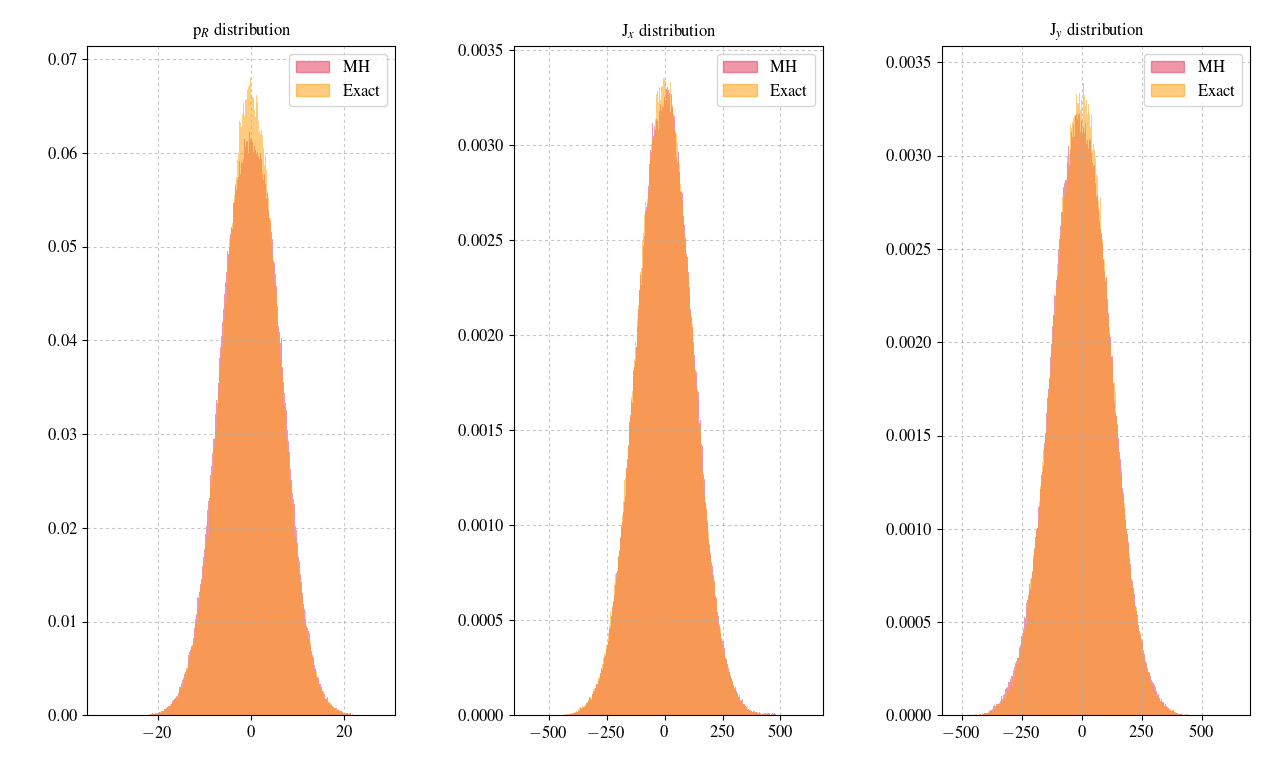
\includegraphics[width=\textwidth]{../pictures/diatomicsMHExactDistributions.png}
	\caption{Распределения переменных $p_R$, $J_x$, $J_y$ для двух атомов с массами $m_{Ar}$ и $m_{CO_2}$ при $T = 300 K$, полученные методом $MH$ и по точным формулам, 500.000 точек, $R$ = 20 бор.}
	\label{fig:pict_mh}
\end{figure}

